%
% Spark reference architectures
% Copyright (C) 2016 Martin Zapletal
%
% This program is free software: you can redistribute it and/or modify
% it under the terms of the GNU General Public License as published by
% the Free Software Foundation, either version 3 of the License, or
% (at your option) any later version.
%
% This program is distributed in the hope that it will be useful,
% but WITHOUT ANY WARRANTY; without even the implied warranty of
% MERCHANTABILITY or FITNESS FOR A PARTICULAR PURPOSE.  See the
% GNU General Public License for more details.
%
% You should have received a copy of the GNU General Public License
% along with this program.  If not, see <http://www.gnu.org/licenses/>.
%

\documentclass[a4paper, 10 pt, conference]{IEEEtran}

\usepackage{graphicx}
\usepackage{interval}
\usepackage{listings}
\usepackage{hyperref}
\usepackage{siunitx}
\usepackage{amsmath}

\sisetup{load-configurations = abbreviations, binary-units = true}
\intervalconfig {
soft open fences ,
separator symbol =; ,
}

\title{Spark Reference Architecture \\ Financial transactions streaming}

\author{Martin Zapletal%$^{1}$% <-this % stops a space
%\thanks{Supported by Cake Solutions Limited}% <-this % stops a space
%\thanks{$^{1}$Martin Zapletal is the CTO at Cake Solutions Inc., 195 Plymout Street, 11201, New York {\tt\small martinz at cakesolutions.net}}%
}


\begin{document}

\maketitle
\thispagestyle{empty}
\pagestyle{empty}

%%%%%%%%%%%%%%%%%%%%%%%%%%%%%%%%%%%%%%%%%%%%%%%%%%%%%%%%%%%%%%%%%%%%%%%%%%%%%%%%
\begin{abstract}
This document describes distributed, large data volume stream processing architecture that was used in a real life production financial transaction processing system. The system receives input data from files at defined times and at the same time continuously ingests data from a streaming integration point, processes and transforms the data as a stream, validates them against known records and finally stores the results.

The document describes architecture, technology choices, explanation of system requirements such as data consistency, integrity, performance, fault tolerance or availability and how the selected technologies and their interoperability fulfil the requirements, focusing on Apache Spark. Finally scenarios where selected technologies and architecture can not be applied due to specific limitations are discussed.
\end{abstract}


%%%%%%%%%%%%%%%%%%%%%%%%%%%%%%%%%%%%%%%%%%%%%%%%%%%%%%%%%%%%%%%%%%%%%%%%%%%%%%%%
\section{Introduction}

\subsection{Spark components}
This reference architecture uses Spark Core, Spark Streaming and Spark SQL.

\subsection{Non Spark components}

Apart from Apache Spark this reference architecture makes use of Cassandra, Kafka, Filesystem, S3 and Elasticsearch.

\subsection{Resource manager}
For automated deployment, infrastructure and operations and resource management Mesosphere Datacenter Operating System (CS/OS) is used.

\section{Reference implementation}

The application receives multiple types of inputs. One are files from other financial institution uploaded at defined times to an integration point and containing a set of transactions. The other one is integration with other systems through Apache Kafka. The records are processed, validated against known data stored in Cassandra database, transformed and finally stored in Cassandra and relevant information sent to integration points with other internal systems. In addition generation of reports from the stored result data is required. The application has strict requirements for uptime, availability, consistency, data integrity, scalability and cost optimisation while ideally using OS technologies. For those reasons Mesosphere DSOS was chosen for infrastructure automation, cluster and resource management.

\section{Main components}

The main components in this architecture are data sources (file source and Apache Kafka), stream processing pipeline and database. High level architecture is displayed on figure~\ref{fig:components}. 

\begin{figure}[hb]
	\begin{center}
		\caption{Components}
		\label{fig:components}
		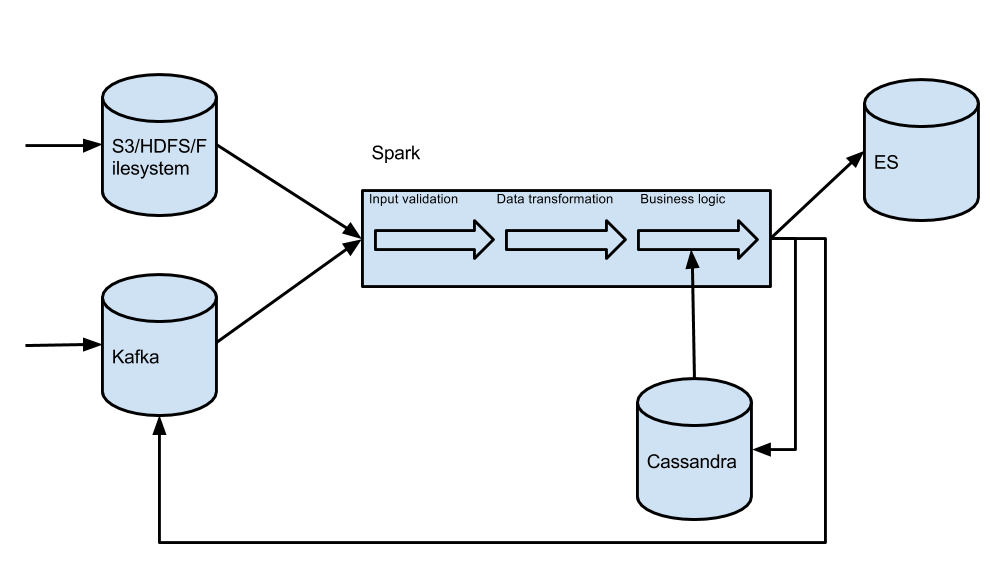
\includegraphics[width=8cm,keepaspectratio]{architecture-diagram.png}
	\end{center}
\end{figure}

\subsection{Data sources}
In this reference architecture two different data sources are used. An input directory is used for historical reasons as an integration point between financial institutions. A file in a known format is uploaded to the directory in defined intervals. Apache Spark file stream source can monitor a directory and process each new file as it is added to the directory. For simplicity of deployment, version upgrades, elasticity, ability to assign very different resources to different types of processed files and financial savings batch processing capability of Apache Spark was preferred.
Apache Kafka is used for integration with other internal systems. Kafka is a distributed log often used for integration for its scalability, reliability, durability, replayability and other attributes. Spark Streaming provides a Kafka input stream and its direct version as options to stream data from Kafka.

\subsection{Stream processing}
After ingesting data from the sources they need to go through a processing pipeline with guarantees satisfying the requirements. The requirements and guarantees provided by Spark are in detail described in next section.
The stream processing pipeline is used for the following purposes.

\subsubsection{Input cleaning and validation}
The inputs are validated. For example the input may not be in the correct format, expected schema invalid, required fields may be missing, outliers may be checked, input data from different publishers standardised and cleaned or other validation done and data filtered.

\subsubsection{Data transformation}
Before processing the data we may need to transform the data into correct format. That may involve transforming from XML/json/cvs/binary or other data format to business logic representation that is easier and safer to work with, query and analyse.

\subsubsection{Business logic implementation}
After the data are in correct format for processing we can apply the actual business logic rules. It may involve queries, real time analytics, aggregations, training and application of machine learning model or asynchronous communication with other systems. In this particular architecture the input data are validated and enriched using records stored in Cassandra database.

\subsubsection{Data storage}
The processed data are stored in a database solution. Firstly, the business logic records are updated using the previously applied business rules. Secondly, an analytics data store is updated with the new records for advanced analytics and search purposes. 

\subsubsection{Result integration}
Enterprise systems are often large distributed application consisting of many services, independent applications and modules. Spark is used to provide updates about the real time processing to the interested services by publishing a stream to Apache Kafka. Kafka is then used as streaming data platform for other systems to subscribe to real time updates with Kafka's strong guarantees.

\section{Streaming data platform}

\begin{figure}[hb]
	\begin{center}
		\caption{Streaming data platform}
		\label{fig:streamingDataPlatform}
		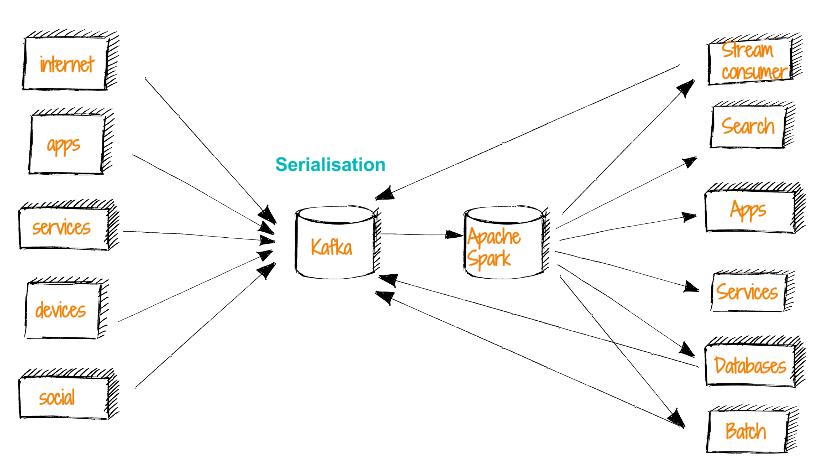
\includegraphics[width=8cm,keepaspectratio]{streaming-data-platform.png}
	\end{center}
\end{figure}

Commonly, ETL and data processing was done in batches and batch processing architectures, supported by Hadoop and similar technologies was common. Due to lack of flexibility and often slow results Lambda Architecture was introduced. It uses batch layer to still deliver correct result and streaming layer to deliver some or partial results quickly.
ETL and batch processes were still often run in intervals capturing a current snapshot of the data to mimic streaming, often due to insufficient access to streaming solutions. The approaches to data processing were questioned with the introduction of Streaming data platform (sometimes called Kappa architecture) in [https://www.oreilly.com/ideas/questioning-the-lambda-architecture] displayed on figure~\ref{fig:streamingDataPlatform}.

This architecture uses a solution that can handle large scale streaming data such as Apache Kafka. Any team, application, system, service, sensors, devices etc. can publish their data into the streaming platform. On the consumer side anyone can subscribe to the streaming data platform and consume the streams they are interested in. They are kept up to date with the latest data using a streaming solution and depend on guarantees a particular streaming solution offers.
The advantages compared to batch processing are obvious. Not only are the same guarantees of batch processing maintained, but the consumers are kept up to date in near real time.
Apache Spark Streaming module fits very well into such architecture with reliable delivery, fault tolerance, throughput, scalability and integration with many other streaming solutions. It is used as a consumer and for transformation, repartitioning of data and preparation for the subscribers to use efficiently as displayed on figure~\ref{fig:streamingDataPlatform}.

\section{Requirements and Spark's guarantees}

\subsection{Data consistency}
The application requires strong consistency guarantees (not in strong serializability database transaction sense sense). The data must always be processed and the result correctly updated. All records from an incoming file or Kafka connector must be processed. 

\subsection{Delivery guarantees}
The application also requires exactly once delivery guarantees. Each element read from either file or Kafka must be delivered exactly once. In distributed environment this is not trivial, because of unbounded delays, lost messages, failed nodes and asynchronous partial failures. In general case durable persistence on both sides of the pipeline is required, because if a message was acknowledged before processing by the receiver, it could result in loss and if it is acknowledged after processing the receiver can receive duplicates (after retry). Exactly once delivery guarantee problem can be reduced to at least once delivery guarantee by using unique identifiers, idempotence or simplified by using probabilistic data structures to filter duplicate data.

Spark provides exactly once delivery guarantee with additional solutions to non replayable sources (replicating the processing pipeline, storing received data immediately into a durable store), parallel recovering from failures optimisations etc.

TODO: COMPLETE http://www.cakesolutions.net/teamblogs/spark-streaming-tricky-parts

\subsection{Fault tolerance}
To fulfil the consistency and delivery requirements fault tolerance is a must. Spark handles node failures, lost data and other common failures in large scale distributed deployments automatically abstracting all that from the application developer.

TODO: COMPLETE (parallel recovery)
Spark Driver program in client mode does not provide resiliency, but in cluster mode 

It is possible to have a hot spare master 

Worker nodes launch and monitors job?s executors. When worker fails, all its child process are also gone. Then the worker process is automatically relaunched, processes restarted and tasks reran. When just the Executor process fails, then it is automatically relaunched by the Worker process and any tasks that were in flight are rescheduled. Stream receivers follows the same resiliency characteristics as 
executors.

\begin{figure}[hb]
	\begin{center}
		\caption{Spark Streaming Failure Impact}
		\label{fig:sparkStreamingFailureImpact}
		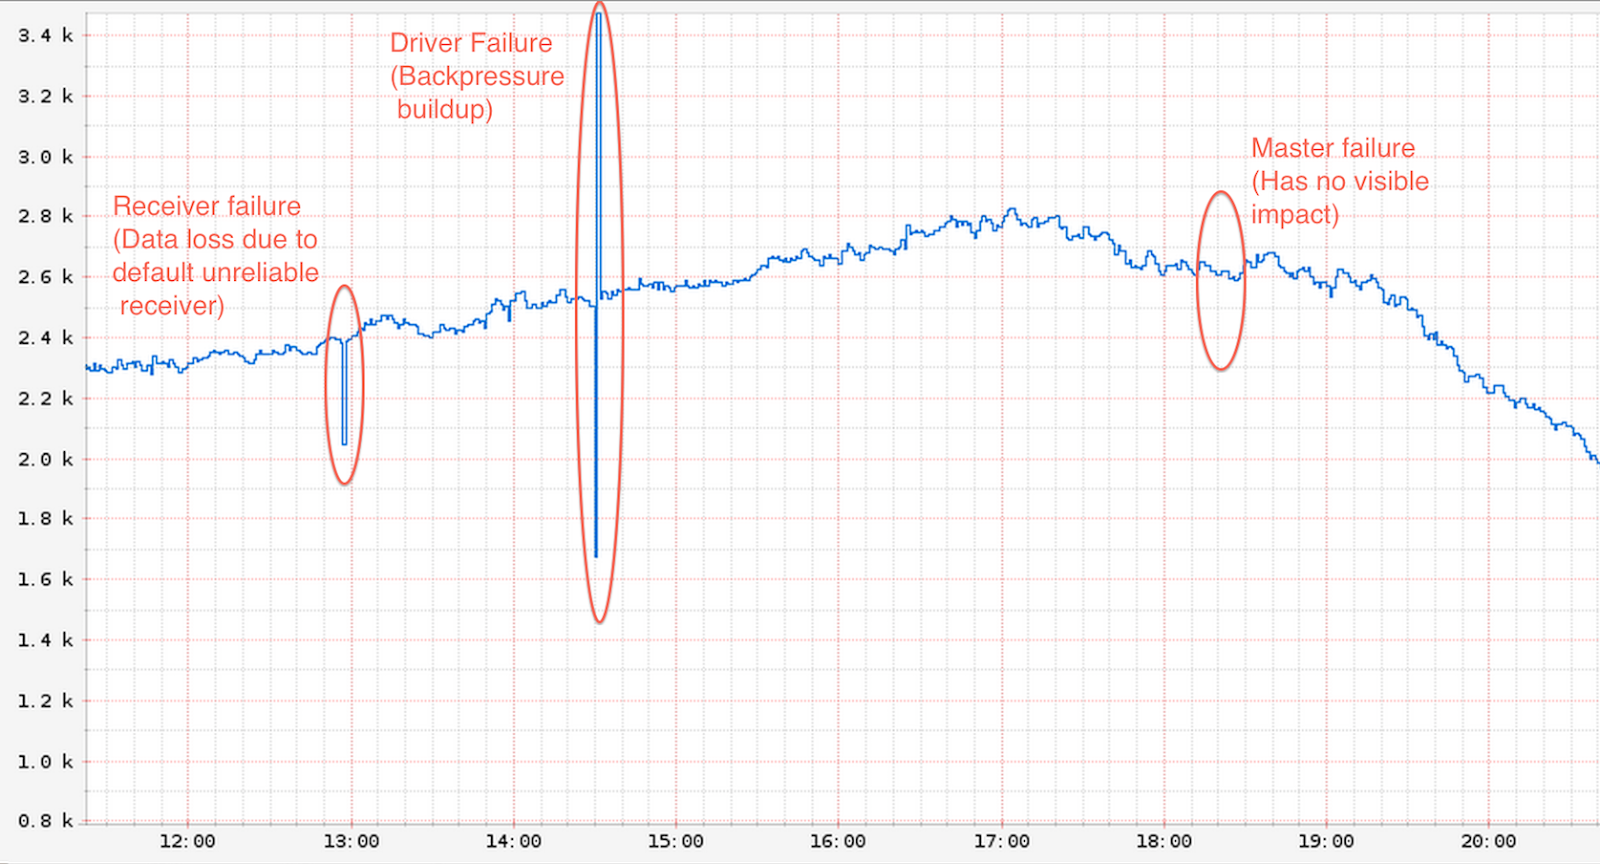
\includegraphics[width=8cm,keepaspectratio]{spark-streaming-failure-impact.png}
	\end{center}
\end{figure}

Failure recovery has impact on the performance ... as displayed on figure~\ref{fig:sparkStreamingFailureImpact}.

\subsection{Order}
Ordering
Event time processing

TODO: COMPLETE

\subsection{Scalability}
The batch part of the pipeline has string scalability guarantees. Different inputs are received at different times and have very different profile of core/ram usage and other resource requirements. Keeping all the resources in the cluster available at all times would be very expensive. The ability to scale the size of the cluster up and down elastically is very important. The pattern could look 

\begin{table}[h]
\caption{Processing times requirements}
\label{tbl:processing-times-requirements}
\begin{center}
  \begin{tabular}{ | l | p{3cm} | }
    \hline
    Between 08:00 and 10:00 & run a defined number of ingestion jobs and a defined number of other transaction ingestion jobs.  \\ \hline
    Between 10:00 and 12:00 & execute ingestion jobs ? as many as the current infrastructure will support. \\ \hline
    At 12:00 & execute a transaction reporting extract using all cluster resorces \\ \hline
    When the above has finished & run housekeeping jobs in parallel ? sharing the cluster resources to prepare for next run \\
    \hline
  \end{tabular}
\end{center}
\end{table}

Spark in cooperation with DC/OS provides capabilities to efficiently utilise provisioned resources. Using e.g. a public cloud infrastructure and utilising the pricing strategy it is possible to achieve significant financial savings.
 
 
TODO: COMPLETE https://docs.google.com/document/d/1jdPtcDyRXWheIQ4MLJpXeK4IoxtUrcThou6LmkUaN28/edit
The stream processing pipeline scaling is 
Elasticity
Dynamic
Dynamic changes to pipeline

\subsection{Latency and throughput}
\subsection{No downtime deployment}
\subsection{Monitoring, logging, operations}
\subsection{Serialisation and versioning}
\subsection{Development tools and visualisation}

\section{Alternatives and competitors}

\section{Conclusion}


\addtolength{\textheight}{-12cm}  % This command serves to balance the column lengths
                                  % on the last page of the document manually. It shortens
                                  % the textheight of the last page by a suitable amount.
                                  % This command does not take effect until the next page
                                  % so it should come on the page before the last. Make
                                  % sure that you do not shorten the textheight too much.

\begin{thebibliography}{99}
\bibitem{apache-cassandra} Apache Cassandra.
\bibitem{apache-spark} Apache Spark.
\end{thebibliography}

\end{document}
